\documentclass[11pt]{article}
\usepackage{amsmath,amssymb,amsmath,amsthm,amsfonts}
\usepackage{latexsym,graphicx}
\usepackage{fullpage,color}
\usepackage{url,hyperref}
\usepackage{natbib}
\usepackage{graphicx,subfigure}
\usepackage{algorithm}
\usepackage{algorithmic}
\usepackage{listings}
\usepackage{xcolor}
\usepackage{color}

\numberwithin{equation}{section}

\pagestyle{plain}

\setlength{\oddsidemargin}{0in}
\setlength{\topmargin}{0in}
\setlength{\textwidth}{6.5in}
\setlength{\textheight}{8.5in}

\newtheorem{fact}{Fact}[section]
\newtheorem{question}{Question}[section]
\newtheorem{lemma}{Lemma}[section]
\newtheorem{theorem}[lemma]{Theorem}
\newtheorem{assumption}[lemma]{Assumption}
\newtheorem{corollary}[lemma]{Corollary}
\newtheorem{prop}[lemma]{Proposition}
\newtheorem{claim}{Claim}[section]
\newtheorem{remark}{Remark}[section]
\newtheorem{definition}{Definition}[section]
\newtheorem{prob}{Problem}[section]
\newtheorem{conjecture}{Conjecture}[section]
\newtheorem{property}{Property}[section]

\def\A{{\bf A}}
\def\a{{\bf a}}
\def\B{{\bf B}}
\def\bb{{\bf b}}
\def\C{{\bf C}}
\def\c{{\bf c}}
\def\D{{\bf D}}
\def\d{{\bf d}}
\def\E{{\bf E}}
\def\e{{\bf e}}
\def\F{{\bf F}}
\def\f{{\bf f}}
\def\g{{\bf g}}
\def\h{{\bf h}}
\def\G{{\bf G}}
\def\H{{\bf H}}
\def\I{{\bf I}}
\def\K{{\bf K}}
\def\k{{\bf k}}
\def\LL{{\bf L}}
\def\M{{\bf M}}
\def\m{{\bf m}}
\def\N{{\bf N}}
\def\n{{\bf n}}
\def\PP{{\bf P}}
\def\Q{{\bf Q}}
\def\q{{\bf q}}
\def\R{{\bf R}}
\def\rr{{\bf r}}
\def\S{{\bf S}}
\def\s{{\bf s}}
\def\T{{\bf T}}
\def\tt{{\bf t}}
\def\U{{\bf U}}
\def\u{{\bf u}}
\def\V{{\bf V}}
\def\v{{\bf v}}
\def\W{{\bf W}}
\def\w{{\bf w}}
\def\X{{\bf X}}
\def\x{{\bf x}}
\def\Y{{\bf Y}}
\def\y{{\bf y}}
\def\Z{{\bf Z}}
\def\z{{\bf z}}
\def\0{{\bf 0}}
\def\1{{\bf 1}}



\def\AM{{\mathcal A}}
\def\CM{{\mathcal C}}
\def\DM{{\mathcal D}}
\def\EM{{\mathcal E}}
\def\GM{{\mathcal G}}
\def\FM{{\mathcal F}}
\def\IM{{\mathcal I}}
\def\JM{{\mathcal J}}
\def\KM{{\mathcal K}}
\def\LM{{\mathcal L}}
\def\NM{{\mathcal N}}
\def\OM{{\mathcal O}}
\def\PM{{\mathcal P}}
\def\SM{{\mathcal S}}
\def\TM{{\mathcal T}}
\def\UM{{\mathcal U}}
\def\VM{{\mathcal V}}
\def\WM{{\mathcal W}}
\def\XM{{\mathcal X}}
\def\YM{{\mathcal Y}}
\def\RB{{\mathbb R}}
\def\RBmn{{\RB^{m\times n}}}
\def\EB{{\mathbb E}}
\def\PB{{\mathbb P}}

\def\TX{\tilde{\bf X}}
\def\TA{\tilde{\bf A}}
\def\tx{\tilde{\bf x}}
\def\ty{\tilde{\bf y}}
\def\TZ{\tilde{\bf Z}}
\def\tz{\tilde{\bf z}}
\def\hd{\hat{d}}
\def\HD{\hat{\bf D}}
\def\hx{\hat{\bf x}}
\def\nysA{{\tilde{\A}_c^{\textrm{nys}}}}

\def\alp{\mbox{\boldmath$\alpha$\unboldmath}}
\def\bet{\mbox{\boldmath$\beta$\unboldmath}}
\def\epsi{\mbox{\boldmath$\epsilon$\unboldmath}}
\def\etab{\mbox{\boldmath$\eta$\unboldmath}}
\def\ph{\mbox{\boldmath$\phi$\unboldmath}}
\def\pii{\mbox{\boldmath$\pi$\unboldmath}}
\def\Ph{\mbox{\boldmath$\Phi$\unboldmath}}
\def\Ps{\mbox{\boldmath$\Psi$\unboldmath}}
\def\ps{\mbox{\boldmath$\psi$\unboldmath}}
\def\tha{\mbox{\boldmath$\theta$\unboldmath}}
\def\Tha{\mbox{\boldmath$\Theta$\unboldmath}}
\def\muu{\mbox{\boldmath$\mu$\unboldmath}}
\def\Si{\mbox{\boldmath$\Sigma$\unboldmath}}
\def\si{\mbox{\boldmath$\sigma$\unboldmath}}
\def\Gam{\mbox{\boldmath$\Gamma$\unboldmath}}
\def\Lam{\mbox{\boldmath$\Lambda$\unboldmath}}
\def\De{\mbox{\boldmath$\Delta$\unboldmath}}
\def\Ome{\mbox{\boldmath$\Omega$\unboldmath}}
\def\Pii{\mbox{\boldmath$\Pi$\unboldmath}}
\def\varepsi{\mbox{\boldmath$\varepsilon$\unboldmath}}
\newcommand{\ti}[1]{\tilde{#1}}
\def\Ncal{\mathcal{N}}
\def\argmax{\mathop{\rm argmax}}
\def\argmin{\mathop{\rm argmin}}

\def\ALG{{\AM_{\textrm{col}}}}

\def\bias{\mathsf{bias}}
\def\var{\mathsf{var}}
\def\sgn{\mathsf{sgn}}
\def\tr{\mathsf{tr}}
\def\rk{\mathrm{rank}}
\def\nnz{\mathsf{nnz}}
\def\poly{\mathrm{poly}}
\def\diag{\mathsf{diag}}
\def\Diag{\mathsf{Diag}}
\def\const{\mathrm{Const}}
\def\st{\mathsf{s.t.}}
\def\vect{\mathsf{vec}}
\def\sech{\mathrm{sech}}

\newcommand{\red}[1]{{\color{red}#1}}



\def\argmax{\mathop{\rm argmax}}
\def\argmin{\mathop{\rm argmin}}

\newenvironment{note}[1]{\medskip\noindent \textbf{#1:}}%
        {\medskip}


\newcommand{\etal}{{\em et al.}\ }
\newcommand{\assign}{\leftarrow}
\newcommand{\eps}{\epsilon}

\newcommand{\opt}{\textrm{\sc OPT}}
\newcommand{\script}[1]{\mathcal{#1}}
\newcommand{\ceil}[1]{\lceil #1 \rceil}
\newcommand{\floor}[1]{\lfloor #1 \rfloor}



\lstset{ %
extendedchars=false,            % Shutdown no-ASCII compatible
language=Python,                % choose the language of the code
xleftmargin=1em,
xrightmargin=1em,
basicstyle=\footnotesize,    % the size of the fonts that are used for the code
tabsize=3,                            % sets default tabsize to 3 spaces
numbers=left,                   % where to put the line-numbers
numberstyle=\tiny,              % the size of the fonts that are used for the line-numbers
stepnumber=1,                   % the step between two line-numbers. If it's 1 each line
                                % will be numbered
numbersep=5pt,                  % how far the line-numbers are from the code   %
keywordstyle=\color[rgb]{0,0,1},                % keywords
commentstyle=\color[rgb]{0.133,0.545,0.133},    % comments
stringstyle=\color[rgb]{0.627,0.126,0.941},      % strings
backgroundcolor=\color{white}, % choose the background color. You must add \usepackage{color}
showspaces=false,               % show spaces adding particular underscores
showstringspaces=false,         % underline spaces within strings
showtabs=false,                 % show tabs within strings adding particular underscores
frame=single,                 % adds a frame around the code
%captionpos=b,                   % sets the caption-position to bottom
breaklines=true,                % sets automatic line breaking
breakatwhitespace=false,        % sets if automatic breaks should only happen at whitespace
%title=\lstname,                 % show the filename of files included with \lstinputlisting;
%                                % also try caption instead of title
mathescape=true,escapechar=?    % escape to latex with ?..?
escapeinside={\%*}{*)},         % if you want to add a comment within your code
%columns=fixed,                  % nice spacing
%morestring=[m]',                % strings
%morekeywords={%,...},%          % if you want to add more keywords to the set
%    break,case,catch,continue,elseif,else,end,for,function,global,%
%    if,otherwise,persistent,return,switch,try,while,...},%
}


\begin{document}

%\setlength{\fboxrule}{.5mm}\setlength{\fboxsep}{1.2mm}
%\newlength{\boxlength}\setlength{\boxlength}{\textwidth}
%\addtolength{\boxlength}{-4mm}


\title{CS583A: Final Exam (Sample Questions)}

\author{{\bf Name}: ~~~~~~~~~\qquad ~~~~~ \qquad~~~~~~~~~}

\date{ }

\maketitle



\paragraph{Policy:}
Books and printed materials are allowed. Do not use electronic divice, including phone, laptop, and tablet.

\paragraph{Hint:} (i) $\frac{\partial  e^a}{\partial a} = e^a$, (ii) $\frac{ \partial \log_e (a) }{\partial a  } = \frac{1}{a}$, (iii) $\frac{ \partial \frac{1}{a} }{\partial a  } = - \frac{1}{a^2}$, and (iv) $\frac{ \partial \cos (a) }{\partial a  } = - \sin (a)$.



\paragraph{Q1 (2\%).} 
Let $\A$ be a real matrix and $\bb$ be a real vector.
To compute the multiplication $\A \bb$ efficiently,
which of the following libraries is the the best choice?
\begin{itemize}
	\item[A.]
	Level 1 BLAS.
	\item[B.]
	Level 2 BLAS.
	\item[C.]
	Level 3 BLAS.
	\item[D.]
	LAPACK.
\end{itemize}


\paragraph{Q2 (2\%).} 
The input shape is $18\times 18$, the pool size is $3\times 3$, and the pooling has no overlap (equivalently, the stride is $3\times 3$).
Then what is the output shape of the pooling?
\begin{itemize}
	\item[A.]
	$3\times 3$.
	\item[B.]
	$6\times 6$.
	\item[C.]
	$15\times 15$.
	\item[D.]
	$16\times 16$.
	\item[E.]
	$18\times 18$.
\end{itemize}



\paragraph{Q3 (2\%).} 
Let $\a = [1, 2, 3, 4, 5]^T$ be a vector.
Let $\bb = \tanh (\a)$, where $\tanh$ is the hyperbolic tangent function.
\underline{Then $\| \bb \|_2^2 < 1$.}
\begin{itemize}
	\item[A.]
	The statement is true.
	\item[B.]
	The statement is false.
\end{itemize}


\paragraph{Q4 (2\%).} 
We want to train a deep convolutional neural network using the CIFAR10 dataset.
Which of the following tricks cannot be applied to improve the test accuracy?
\begin{itemize}
	\item[A.]
	Using dropout regularization.
	\item[B.]
	Using data augmentation.
	\item[C.]
	Using ensemble method.
	\item[D.]
	Using multi-task learning.
\end{itemize}


\paragraph{Q5 (2\%).} 
We use mini-batch SGD with momentum to solve a softmax classifier model.
We use different settings of batch size, $b$, and plot the \textbf{objective function value} against \textbf{epochs} in the figure below.
All the other hyper-parameters in the algorithms have been fine-tuned.
\underline{The figure indicates that MB-SGD with $b=8$ is very likely better than $b=64$ in this case.}
\begin{itemize}
	\item[A.]
	The statement is true.
	\item[B.]
	The statement is false.
\end{itemize}

%---------------------------------Figure---------------------------------%
\begin{figure*}[h]
	\begin{center}
		\vspace{-5mm}
		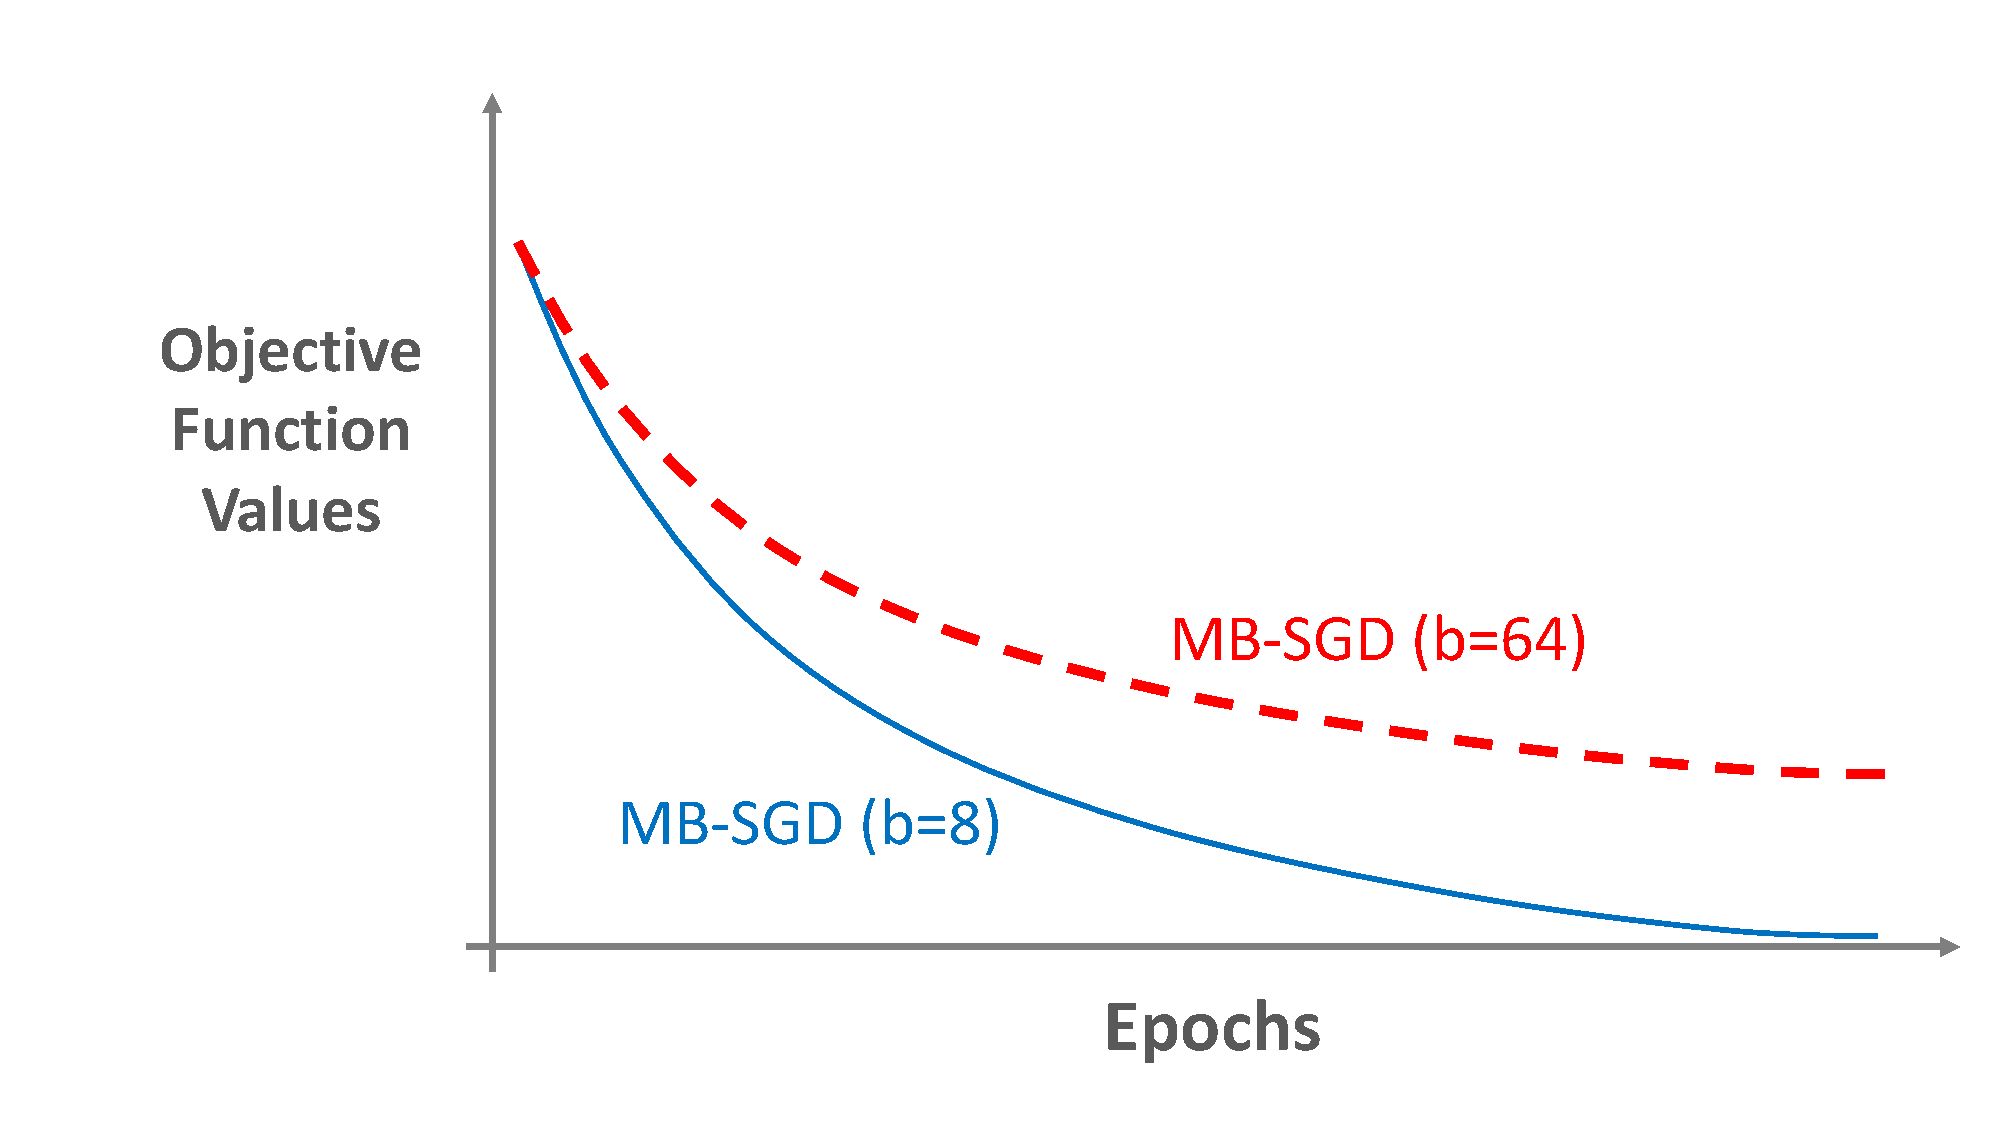
\includegraphics[width=0.5\textwidth]{figure/epochs.pdf}
		\vspace{-4mm}
	\end{center}
\end{figure*}
%---------------------------------Figure---------------------------------%



\paragraph{Q6 (2\%).} 
Suppose we seek to predict increment (either positive or negative) of a stock's price based on its prices in the past.
Which of the followings is the best choice for the activation function of the output layer?
\begin{itemize}
	\item[A.]
	No activation function (equivalently, the identity function).
	\item[B.]
	Rectified linear unit (ReLU).
	\item[C.]
	Logistic function.
	\item[D.]
	Softmax function.
	\item[D.]
	Tanh function.
\end{itemize}



\paragraph{Q7 (2\%).} 
We use a deep learning model to predict whether a customer's review is positive or negative.
We tokenize the reviews in the word-level and thus need an embedding layer to convert words to vectors.
Upon the embedding layer, we build RNN layers and other types of layers.
We find serious overfitting because the dataset has merely 10,000 samples.
Which of the followings is the best improvement?
\begin{itemize}
	\item[A.]
	Pretraining the embedding layer using a big dataset.
	\item[B.]
	Using Bi-LSTM to replace SimpleRNN or LSTM.
	\item[C.]
	Combing self-attention with RNN.
	\item[D.]
	Using stacked-LSTM to increase the model capacity.
\end{itemize}




\paragraph{Q8 (2\%).} 
The following implements a convolutional neural network.
The code has a major problem.
How can we make correction?
\begin{itemize}
	\item[A.]
	Remove the second convolutional layer (Lines 10 to 12), because it is not useful.
	\item[B.]
	Put the batch normalization layers (Lines 8 and 11) after the activations (Lines 9 and 12).
	\item[C.]
	Put the batch normalization layers (Lines 8 and 11) before the convolutions (Lines 7 and 10).
	\item[D.]
	Put the dropout layer (Line 18) before the first dense layer (Line 16).
	\item[E.]
	Put the dropout layer (Line 18) before the second dense layer (Line 17).
\end{itemize}



\begin{lstlisting}
from keras import models
from keras.layers import Input, Conv2D, MaxPooling2D, Activation
from keras.layers import BatchNormalization, Flatten, Dense, Dropout

input_img = Input((128, 128, 3))

x = Conv2D(32, (3, 3))(input_img)
x = BatchNormalization()(x)
x = Activation('relu')(x)
x = Conv2D(32, (3, 3))(x)
x = BatchNormalization()(x)
x = Activation('relu')(x)
x = MaxPooling2D((2, 2))(x)

x = Flatten()(x)
x = Dense(128, activation='relu')(x)
x = Dense(256, activation='relu')(x)
x = Dropout(0.5)(x)
x = Dense(10, activation='softmax')(x)

model = models.Model(input_img, x)
\end{lstlisting}
\vspace{3mm}


\paragraph{Q9 (2\%).} 
The following implements a convolutional neural network.
The code is incorrect.
How can we make correction?
\begin{itemize}
	\item[A.]
	The activation in Line 7 should be removed.
	\item[B.]
	The activation layer (Line 9) should be removed.
	\item[C.]
	The batch normalization layer (Line 8) should be place after the pooling layer (Line 10).
	\item[D.]
	The dropout layer (Line 12) should be placed after Line 13 and before Line 14.
\end{itemize}


\begin{lstlisting}
from keras import models
from keras.layers import Input, Conv2D, BatchNormalization, Activation
from keras.layers import MaxPooling2D, Flatten, Dropout, Dense

input_img = Input((28, 28, 3))

x = Conv2D(32, (3, 3), activation='relu')(input_img)
x = BatchNormalization()(x)
x = Activation('relu')(x)
x = MaxPooling2D((2, 2))(x)
x = Flatten()(x)
x = Dropout(0.5)(x)
x = Dense(1000, activation='relu')(x)
x = Dense(10, activation='relu')(x)

model = models.Model(input_img, x)
\end{lstlisting}
\vspace{3mm}





\paragraph{Q10 (2\%).} 
{\bf (Fill the blank.)}
The training set contains $1,000$ samples.
We train a neural network using mini-batch SGD.
One epoch amounts to $50$ iterations.
What is the batch size? \\
The batch size is \underline{~\qquad\qquad\qquad~}. \\




\paragraph{Q11 (2\%).} 
{\bf (Fill the blank.)}
What is the output of the following Python program?\\
Answer: \underline{~\qquad\qquad\qquad~}
%ANSWER: 3



\begin{lstlisting}
import numpy
a = numpy.random.rand(3, 5) # generate a random matrix
b = numpy.random.rand(5, 10) # generate a random matrix
c = numpy.dot(a, b)
print(c.shape[0])

\end{lstlisting}
\vspace{3mm}


\paragraph{Q12 (12\%).} 
{\bf (Fill the blanks.)}
The following code builds a neural network for sentiment analysis.
\begin{itemize}
	\item 
	Line 10 is an embedding layer. 
	What is the output shape of this layer?\\
	Answer: \underline{~\qquad\qquad\qquad~}
	%ANSWER: 100, 20
	\item 
	What is (roughly) the number of parameters in the embedding layer?\\
	Answer: \underline{~\qquad\qquad\qquad~}
	%ANSWER: 200,000
	\item 
	Line 11 is a SimpleRNN layer. 
	What is the output shape of this layer?\\
	Answer: \underline{~\qquad\qquad\qquad~}
	%ANSWER: 50
	\item 
	What is (roughly) the number of parameters in the SimpleRNN layer?\\
	Answer: \underline{~\qquad\qquad\qquad~}
	%ANSWER: around 3550 (= shape(h) * []shape(h) + shape(x)] + shape(h))
	\item 
	Line 12 is a dense layer. 
	What is the output shape of this layer?\\
	Answer: \underline{~\qquad\qquad\qquad~}
	%ANSWER: 1
	\item 
	What is (roughly) the number of parameters in the dense layer?\\
	Answer: \underline{~\qquad\qquad\qquad~}
	%ANSWER: 51
\end{itemize}



\begin{lstlisting}
from keras.models import Sequential
from keras.layers import SimpleRNN, Embedding, Dense

voc_size = 10000 
shape_x = 20 
seq_length = 100 
shape_h = 50

model = Sequential()
model.add(Embedding(voc_size, shape_x, input_length=seq_length)) 
model.add(SimpleRNN(shape_h, return_sequences=False))
model.add(Dense(1, activation='sigmoid'))
\end{lstlisting}
\vspace{3mm}






\paragraph{Q13 (12\%).} 
The following code builds a convolutional neural network.
\begin{itemize}
	\item 
	Line 5 is a convolutional layer with $1\times 1$ convolutions. 
	What is the output shape of this layer?\\
	Answer: \underline{~\qquad\qquad\qquad~}
	%ANSWER: 100, 100, 10
	\item 
	What is (roughly) the number of parameters in the convolutional layer (Line 5)?\\
	Answer: \underline{~\qquad\qquad\qquad~}
	%ANSWER: around 410
	\item 
	Line 8 is a convolutional layer with $3\times 3$ convolutions. 
	What is the output shape of this layer?\\
	Answer: \underline{~\qquad\qquad\qquad~}
	%ANSWER: 100, 100, 10
	\item 
	What is (roughly) the number of parameters in the convolutional layer (Line 8)?\\
	Answer: \underline{~\qquad\qquad\qquad~}
	%ANSWER: around 910
	\item 
	Line 13 is a pooling layer. 
	What is the output shape of this layer?\\
	Answer: \underline{~\qquad\qquad\qquad~}
	%ANSWER: 100, 100, 40
	\item 
	What is (roughly) the number of parameters in the pooling layer (Line 13)?\\
	Answer: \underline{~\qquad\qquad\qquad~}
	%ANSWER: 0
\end{itemize}





\begin{lstlisting}
from keras.layers import Input, Conv2D, MaxPooling2D, concatenate

x_input = Input(shape=(100, 100, 40))

tower1 = Conv2D(10, (1,1), padding='same', activation='relu')(x_input)

tower2 = Conv2D(10, (1,1), padding='same', activation='relu')(x_input)
tower2 = Conv2D(10, (3,3), padding='same', activation='relu')(tower2)

tower3 = Conv2D(10, (1,1), padding='same', activation='relu')(x_input)
tower3 = Conv2D(10, (5,5), padding='same', activation='relu')(tower3)

tower4 = MaxPooling2D((3,3), strides=(1,1), padding='same')(x_input)
tower4 = Conv2D(10, (1,1), padding='same', activation='relu')(tower4)

x_output = concatenate([tower1, tower2, tower3, tower4], axis = 3)
\end{lstlisting}
\vspace{3mm}




\paragraph{Q14 (6\%).} 
A question based on the textbook.



\paragraph{Q15 (10\%).} 
A matrix calculus question analogous to those in the quiz.




%\vspace{3mm}
%\begin{lstlisting}
%import numpy
%
%def rfm(x, s, sigma):
%	n, d = x.shape
%	a = numpy.random.standard_normal((d, s)) / sigma
%	b = numpy.random.rand(1, s) * (2 * numpy.pi)
%	c = numpy.dot(x, a) + b
%	h = numpy.cos(c) * numpy.sqrt(2/s)
%	return h
%\end{lstlisting}
%\vspace{3mm}

%\newpage
%\bibliographystyle{plain}
%
%%\markboth{\bibname}{\bibname}
%\bibliography{matrix}


\end{document}
